\startprefacepage

Оптимизацией в математике называется задача нахождения экстремума целевой функции в 
некоторой области конечномерного векторного пространства, ограниченной набором линейных 
и/или нелинейных равенств и/или неравенств.

В процессе проектирования ставится обычно задача определения наилучших, в некотором смысле, 
структуры или значений параметров объектов. Такая задача называется оптимизационной. 
Если оптимизация связана с расчётом оптимальных значений параметров при заданной структуре 
объекта, то она называется параметрической оптимизацией. Задача выбора оптимальной структуры 
является структурной оптимизацией.\cite{wiki_opt}

Стандартная математическая задача оптимизации формулируется таким образом. Среди элементов $x$, 
образующих множество $X$, найти такой элемент $x*$, который доставляет минимальное значение 
$f(x*)$ заданной функции $f(X)$.

Многокритериальная оптимизация или программирование — это процесс одновременной оптимизации 
двух или более конфликтующих целевых функций в заданной области определения. Задача 
многокритериальной оптимизации состоит в поиске вектора целевых переменных, удовлетворяющего 
наложенным ограничениям и оптимизирующего векторную функцию, элементы которой соответствуют 
целевым функциям. Эти функции образуют математическое описание критерия удовлетворительности 
и, как правило, взаимно конфликтуют. Отсюда, «оптимизировать» означает найти такое решение, 
при котором значение целевых функций были бы приемлемыми для постановщика задачи. \cite{wiki_multiopt}

В данной работе в качестве критерия оптимальности рассматривается \textit{эффективность по Парето}. 
Эффективность по Парето — такое состояние системы, при котором значение каждого частного 
показателя, характеризующего систему (например, каждой из оптимизируемых функций), не может 
быть улучшено без ухудшения других. Множество состояний системы, оптимальных по Парето, 
называют «множеством Парето», «множеством альтернатив, оптимальных в смысле Парето», 
либо «множеством Парето-оптимальных альтернатив». Используются также термины «компромиссные», 
«неулучшаемые» альтернативы. \cite{wiki_pareto}

	\begin{figure}[h!]
		\center{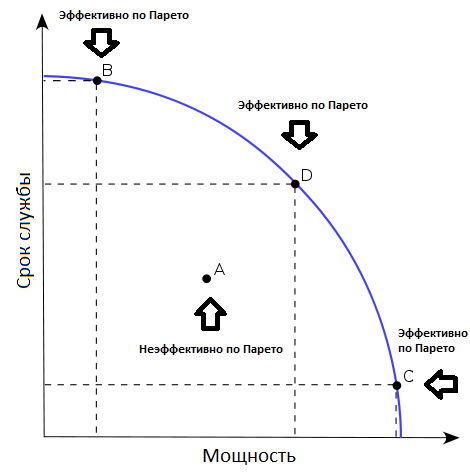
\includegraphics[scale=1]{img/par1}}
		\caption{Пример кривой Парето}
		\label{pict:par1}
	\end{figure}

При выполнении многокритериальной оптимизации, как правило, используется процедура 
\textit{недоминирующей сортировки}. \cite{deb_nsga2}
	
Говорят,  что  в K-мерном  пространстве  точка $A = (a_1, ..., a_K)$ доминирует  над  
точкой $B = (b_1,  ..., b_K)$, когда для $1 \le i \le K $ выполняется неравенство 
$a_i \le b_i $ и существует $j$, такое что $a_j < b_j $.

Недоминирующей сортировкой точек в K-мерном пространстве называется процедура, в результате которой:
\begin{enumerate}
\item Точки, над которыми не доминирует ни одна точка, помечаются \textit{рангом} 0;
\item Точки, над которыми доминирует хотя бы одна точка ранга 0, помечаются рангом 1;
\item Точки, над которыми доминирует хотя бы одна точка ранга i–1, помечаются рангом i.
\end{enumerate}

В результате выполнения недоминирующей сортировки исходное множество точек разбивается на 
\textit{фронты Парето}. Фронтом Парето (или \textit{уровнем недоминирования}) называется 
множество точек, являющихся Парето-оптимальными друг относительно друга. Каждый уровень
недоминирования характеризуется рангом точек, которые в нем содержатся.
Фронт Парето нулевого ранга является множеством точек, оптимальных по Парето.

Целью данной работы является разработка структуры данных, поддерживающей корректную 
структуру уровней недоминирования при добавлении новой точки в двумерном пространстве.
В рамках данной работы предложен алгоритм, позволяющий добавлять или удалять точку за 
линейное ($O(N)$, где $N$ - суммарное количество точек на всех уровнях недоминирования)
время. Использование данной структуры данных позволяет эффективно реализовать 
инкрементальный алгоритм многокритериальной оптимизации \textit{NSGA-II}. 
\cite{max_me_ss_nsga2}.
